% !Mode:: "TeX:UTF-8"
\chapter{绪论}

\section{研究背景}

截至2016年3月,全球最大社交网络平台Facebook活跃用户量已经突破15.9亿。中国最大的社交媒体微博用户也早在2013年突破了6亿用户,国际知名社交平台Twitter也在2016年突破了13亿的注册用户量。随着这些在线社交网络的迅猛发展以及移动智能电话的大规模普及,社交网络分析引起了越来越多的来自计算机、社会学、数学等领域的学者广泛关注。社交网络的原始定义\upcite{刘军2004社会网络分析导论,ccaggarwalintrosocial}来自于社会学,表示社会角色以及其交互关系的集合。而社会角色可以定义为独立的个人,也可以定义为家庭、学校或者国家等社会群体。而社会角色之间的的联系,则可以是任何无形(如两个人之间的朋友关系)或者有形(如国与国之间的合作)的交互关系,这些关系完全都可以由研究问题的学者自己定义。因此,由多个点(即社会角色)以及表示各个点之间关系(即为交互关系)的边所构成的网络,即为社交网络。在我们所生活的世界中,社交网络无处不在,如Email网络、学术网络或手机电话联系网络。虽然互联网的发展,出现了许多的在线社交网络,如Facebook、Twitter、Weibo等等。这一系列的社交网络的兴起促进了海内外各个领域的学者对其的研究,而其研究结果又被用到广告营销、社会服务、公共安全等各种不同的领域。如图1.1即为一个来自Friendster网站的一个社交网络实例。图中可以看到,每个人都是一个点,而每条边表示两个人之间为朋友关系,将它们整体结合起来就构成了一个社交网络。

\begin{figure}[!ht]
    \centering
    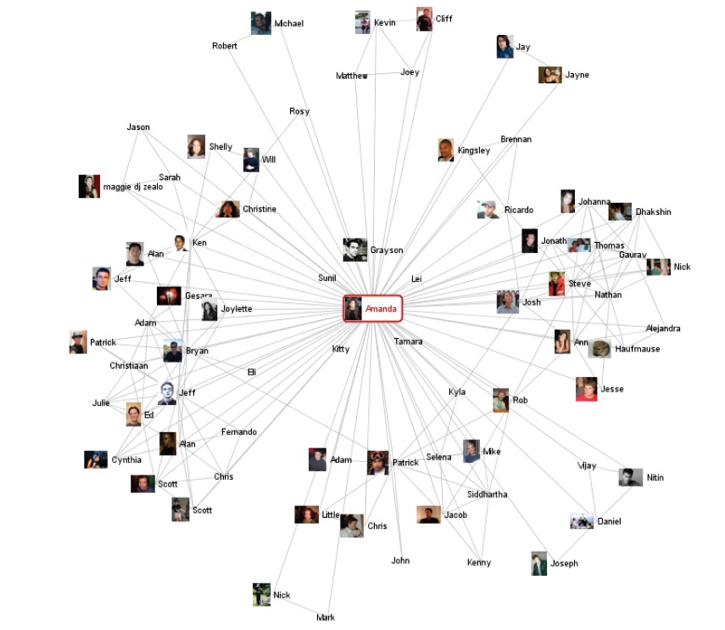
\includegraphics[]{figure/friends.png}
    \caption{来自Friendster网站的社交网络实例\upcite{heer2005vizster}}
    \label{fig-friends}
\end{figure}


在以前的研究中,研究人员主要以在线社交网络为主要研究对象。但在移动互联网出现以前,用户只能通过Web页面登录到相应的社交网站。因此,以前的大多数研究都将重点放在了社交层次的用户交互上,而脱离于现实世界,从而限制了研究人员的研究思路与研究方法。但这几年,随着移动互联网的迅猛发展,越来越多的用户开始在移动终端使用相应的服务。同时,移动开发者也开发了很多基于地理位置服务(LBS, Location Based Service)的移动应用。这一切使得研究社会网络有了新的方向与思路。移动社交网络(Mobile Social Network)是一种以移动终端为媒介、基于地理位置的社会网络。该网络相对于传统的社交网络更偏重于虚拟社会网络与现实世界之间的交互与联系,从而更加接近现实生活中的网络,从而研究者能研究的内容更加广泛、更加贴切现实生活中的实际情况。图1.2则展示了一个典型的移动社交网络。对于该网络中的用户来说,用户之间的虚拟联系(如两人是否为朋友关系)以及他们之间的联系属性构成了社交拓扑图。而对于现实生活中的用户来说,他们在现实世界中具有一定的时间、空间特征,而他们的位置轨迹以及关联等则构成了一幅位置移动图。在传统的社交网络研究中,研究者要么将重点放在社交拓扑图上,要么则主要研究用户之间的位置移动,很少有考虑两者之间的内在联系与共性。而移动社交网络研究中,研究者会同时研究用户的社交与位置轨迹等信息,将虚拟的社会网络与现实的物理世界有机地结合起来,从而能有效的研究用户虚拟世界与现实世界之间的内在共同特征与联系,更加真实的反映用户在现实世界中的行为与特征,为广告投放、社会服务等领域提供了更精准的信息与数据支撑。

\begin{figure}[!ht]
	\centering
	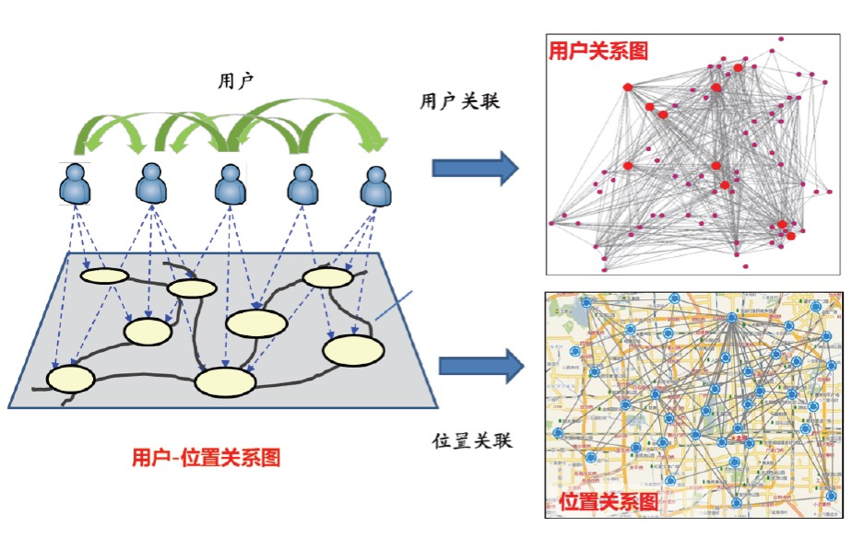
\includegraphics[]{figure/msn.png}
	\caption{移动社交网络}
	\label{fig-msn}
\end{figure}


当前,因为智能手机的大规模普及,和社交媒体(如Facebook、微博等)的飞速发展,很多用户选择在移动端发状态或者消息。许多类似的应用在发状态消息的时,提供了是否要共享地理位置信息的选项。但很多用户基于隐私安全等考虑,并不愿意共享他们的地理位置,因此该数据的位置信息等大多处于缺失状态,很难构建用户的整个地理位置轨迹分布等信息。另外一点,虽然有用户在发状态时选择了共享他们的地理位置信息,但该模式很少和其他用户进行交流、通讯,因此实际上该交互模式中虚拟社交层次与地理交互层次是隔开的,研究者很少能够使用该数据来挖掘两者之间的内在联系,更不能挖掘他们之间的交互特征。因此,本文研究所采用的是移动手机通话数据。在移动社交网络中,移动通话数据具有其它数据不具备的优势,它记录丰富,时空信息完整,采样规律并且频繁,覆盖的人群阶层广泛,能有效的将用户的社交关系与地理轨迹交互联系起来。根据工信部2014年通讯运营业统计公报,我国截至2014年年底移动手机通话用户数量已经达到12.86亿户,普及率达到94.5部/百人\upcite{mobilereport},并且增长十分迅速。如图1.3,可以看出这些年来我国居民拥有的移动终端的数目增加迅速,覆盖面越来越广。平均情况下已经接近人手一部的水平。因此使用移动通话数据网络具有非常高的普适性和广泛性(而其它较大线上社交网络,如微博、Facebook、Twitter等并不具有这些特点)。随着移动通话数据的进一步爆发式增长,基于移动通话数据的移动社交网络研究分析必将更加流行,当然也会带来了更大的机遇和挑战。


\begin{figure}[!ht]
	\centering
	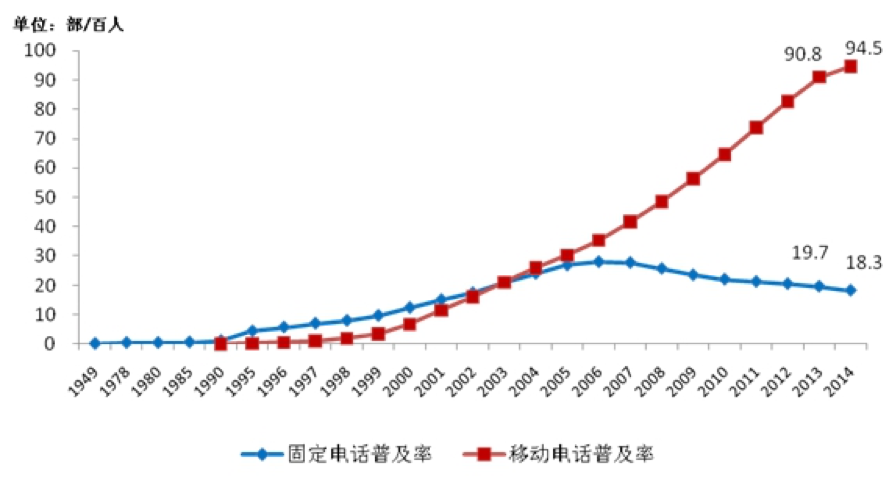
\includegraphics[scale=1,width=0.9\textwidth]{figure/mobileinc.png}
	\caption{1949-2014年固定电话、移动电话用户发展情况}
	\label{fig-mobileinc}
\end{figure}


目前,移动社交网络的研究主要包括对社交网络中人群的画像识别、行为识别、关系预测以探讨社交网络与真实时空之间的关系。这些相关的研究在个性化推荐、用户轨迹预测、可疑用户监测等领域有着广泛的应用。例如在广告营销方面,确定了用户画像,就可以针对特定的用户人群投放更加精准的广告。另外,在追踪和调查犯罪嫌疑人的时候,我们确定了犯罪嫌疑人以及周围的社交关系,就能进一步的帮助相关执法机构缩小侦查范围,帮助公安机关迅速确定犯罪嫌疑人。

随着手机实名制的普及,越来越多的用户在运营商等急了个人的身份信息。当前很多家庭或者公司办理了家庭套餐、工作套餐等业务。这一套餐为我们精准把握用户之间的关系提供了数据支撑。尽管我国在大力推广手机实名制,但是全国仍然有将近3亿的用户的信息处于缺失状态。因此,如何利用这些信息来推断人与人之间的关系,即是当前社会的迫切需求,也是本文的挑战之一。


%\section{国内外研究现状}
 
%社交关系识别可以归结于关系预测等社交网络领域的经典研究问题。




\section{本文主要内容}

本文主要利用移动通话数据构建了一个移动社交网络,并对该网络中用户与用户之间的社交关系进行了探讨。其主要内容如下:

\begin{enumerate}
\item[1)]问题定义及介绍 \\
本文从当前研究移动社交网络的热点出发,定义了我们所要研究的问题,即关系识别在移动社交网络中的研究。除此之外,详细介绍了我们的移动社交网络的数据以及该网络的特点。

\item[2)] 移动社交网络特征 \\
本文针对我们所研究的移动社交网络的特点,结合社会学、空间学等理论,提出了一系例具有时间、空间、网络结构和用户交互的特征,并对这些特征在真实数据集上进行验证了其有效性。

\item[3)] 关系识别模型 \\
本文针对我们所研究的问题,在基于概率图等模型的基础上,提出了我们用于关系识别的模型,并在真实数据集上测试了我们的算法,具有较高的识别准确率。

\item[4)] 结果分析及改进 \\
本文针对模型的结果,详细的分析了各类因素对结果的影响,并针对这些结果分析了背后所存在的原因,并给出了一个高效并行的算法实现。
\end{enumerate}



\section{本文组织安排}

本文共六章,总体的组织安排如下:

第一章为绪论,阐述了本文的研究背景以及研究意义,并介绍了当前国内外关系识别的研究现状。最后简单介绍了一下本文研究的主要内容。

第二章为基于社交网络的的研究与挑战,介绍了当前常用于该领域的几种模型。

第三章为针对移动社交网络所提出有特色的特征,介绍完了我们综合时间、空间、网络结构等方面所提出的特征。

第四章为我们针对所提出特征而建立的模型,该模型是基于概率图模型并针对我们的特征而构建的。

第五章为结果分析,针对我们模型的结果进行详细分析与并分析了对比实验。

第六章为总结与展望,主要总结了本文的研究工作与创新点,同时也指出了当前研究工作的不足,并提出了未来的研究方向。











